% Exam Template for UMTYMP and Math Department courses
%
% Using Philip Hirschhorn's exam.cls: http://www-math.mit.edu/~psh/#ExamCls
%
% run pdflatex on a finished exam at least three times to do the grading table on front page.
%
%%%%%%%%%%%%%%%%%%%%%%%%%%%%%%%%%%%%%%%%%%%%%%%%%%%%%%%%%%%%%%%%%%%%%%%%%%%%%%%%%%%%%%%%%%%%%%

% These lines can probably stay unchanged, although you can remove the last
% two packages if you're not making pictures with tikz.
\documentclass[11pt]{exam}
\RequirePackage{amssymb, amsfonts, amsmath, latexsym, verbatim, xspace, setspace}
\RequirePackage{tikz, pgflibraryplotmarks}

% By default LaTeX uses large margins.  This doesn't work well on exams; problems
% end up in the "middle" of the page, reducing the amount of space for students
% to work on them.
\usepackage[margin=1in]{geometry}


% Here's where you edit the Class, Exam, Date, etc.
\newcommand{\class}{Principles of Operating Systems}
\newcommand{\term}{Winter 2017}
\newcommand{\examnum}{Final}
\newcommand{\examdate}{03/22/2017}
\newcommand{\timelimit}{8:00am - 10:00am}

% For an exam, single spacing is most appropriate
\singlespacing
% \onehalfspacing
% \doublespacing

% For an exam, we generally want to turn off paragraph indentation
\parindent 0ex

\begin{document} 

% These commands set up the running header on the top of the exam pages
\pagestyle{head}
\firstpageheader{}{}{}
\runningheader{\class}{\examnum\ - Page \thepage\ of \numpages}{\examdate}
\runningheadrule

\begin{flushright}
\begin{tabular}{p{2.8in} r l}
\textbf{\class} & \textbf{Name (Print):} & \makebox[2in]{\hrulefill}\\
\textbf{\term} &&\\
\textbf{\examnum} &&\\
\textbf{\examdate} &&\\
\textbf{Time Limit: \timelimit} & & \\
\end{tabular}\\
\end{flushright}
\rule[1ex]{\textwidth}{.1pt}




%\begin{minipage}[t]{3.7in}
%\vspace{0pt}
\begin{itemize}

\item \textbf{Don't forget to write your name on this exam.} 

\item \textbf{This is an open book, open notes exam. But no online or 
    in-class chatting.  } 

    
\item \textbf{Ask me if something is not clear in the questions.}

\item \textbf{Organize your work}, in a reasonably neat and coherent way, in
the space provided. Work scattered all over the page without a clear ordering will 
receive very little credit.  

\item \textbf{Mysterious or unsupported answers will not receive full
credit}.  A correct answer, unsupported by explanation will receive no credit; 
an incorrect answer supported by substantially correct explanations might still 
receive partial credit.

\item If you need more space, use the back of the pages; clearly indicate when you have done this.
\end{itemize}

%Do not write in the table to the right.
%\end{minipage}
%\hfill

%\begin{minipage}[t]{2.3in}
%\vspace{0pt}
%\cellwidth{3em}
%\gradetablestretch{2}
\vqword{Problem}
\addpoints % required here by exam.cls, even though questions haven't started yet.	
\gradetable[v]%[pages]  % Use [pages] to have grading table by page instead of question

%\end{minipage}
\newpage % End of cover page

%%%%%%%%%%%%%%%%%%%%%%%%%%%%%%%%%%%%%%%%%%%%%%%%%%%%%%%%%%%%%%%%%%%%%%%%%%%%%%%%%%%%%
%
% See http://www-math.mit.edu/~psh/#ExamCls for full documentation, but the questions
% below give an idea of how to write questions [with parts] and have the points
% tracked automatically on the cover page.
%
%
%%%%%%%%%%%%%%%%%%%%%%%%%%%%%%%%%%%%%%%%%%%%%%%%%%%%%%%%%%%%%%%%%%%%%%%%%%%%%%%%%%%%%

\begin{questions}

% Basic question
\addpoints
\question File system


Xv6 lays out the file system on disk as follows:

\begin{figure}[h] \centering
  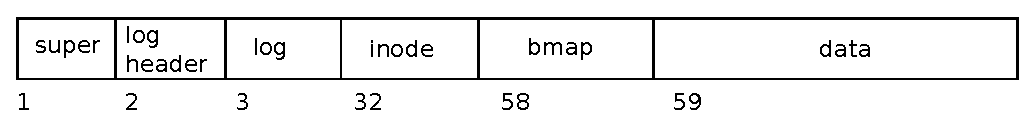
\includegraphics[width=0.8\columnwidth]{figs/fs}
  \label{fig:ramengine-decomposed-app}

\end{figure}

Block 1 contains the super block. Blocks 2 through 31 contain the log header
and the log. Blocks 32 through 57 contain inodes. Block 58 contains the bitmap
of free blocks. Blocks 59 through the end of the disk contain data blocks.

Ben modifies the function bwrite in bio.c to print the block number of each
block written.

Ben boots xv6 with a fresh fs.img and types in the
command ln cat cat2. This command creates a symbolic link cat2 to file cat.
This command produces the following trace:

\begin{verbatim} 
$ ln cat cat2
write 3
write 4
write 2
write 32
write 59
write 2
$
\end{verbatim}

\begin{parts} 

\part[5] Why is block 2 written twice? 

Block 2 is written first time to record the fact that two blocks are in the
log, i.e. the in−memory log header is written to disk. After the entire log is
installed, the header is updated the second time to indicate the fact that
transaction is fully commited, and no recovery is needed in case of a system
crash. 

\vfill

\part[5] Briefly explain what block 32 contains in the above trace. Why is it written?

Block 32 contains the inode for the cat file. Since we're creating a simbolic
link, the inode reference count is incremented to 2 (the same inode is
referenced by both ``/cat'' and ``/cat2'', and is written back to disk.  

\vfill

\newpage

\part[5] What does block 3 contain? 

Block 3 contains the copy of block 32, i.e., the inode that contains ``/cat''
and ``/cat2'' 

\vfill 


\part[5] If writes to 32 and 59 are reordered like below, will it violate correctness of the file system, explain why? 

\begin{verbatim}
$ ln cat cat2
write 3
write 4
write 2
write 59
write 32
write 2
$
\end{verbatim}

No, since we install all the writes atomically, i.e., all or none, the write
order doesn't matter. 

\vfill
\end{parts}

\newpage
\addpoints
\question Memory management. 

\begin{parts}
\part[5] Explain organization of the xv6 memory allocator. 

The xv6 memory allocator is implemented as a linked list of pages. On
allocation, an element of the list that is pointed by the head pointer is
removed from the list. The virtual address of the list element is used as the
allocated address and is returned to the caller. 

\vfill

    
\part[5] Why do you think xv6 does not have buddy or slab allocators? Under 
what conditions you would have to add these allocators to the xv6 kernel? 


Xv6 doesn't implement buddy and slab allocators, since it doesn't really
allocate any memory for kernel data structures. I.e., all data structures used
by the kernel are statically preallocated as arrays with max number of
elemements, e.g., 

\begin{verbatim} struct proc proc[NPROC]; \end{verbatim}

Xv6 allocates only pages of memory for user-level processes, kernel stacks, and
page tables. If xv6 allocated kernel data structures dynamically, it would
require a hierarchy of allocators, malloc on top of slab, on top of buddy to
serve allocations of variable size. 

\vfill


\end{parts}

\newpage
\addpoints
\question Synchronization

\begin{parts}

\part[10] The code below is the xv6's sleep() function. Remember the whole idea
of passing a lock inside sleep() is to make sure it is released before the
process goes to sleep (otherwise it will never be woken up). However, it looks
like that if the lock passed inside sleep is ptable.lock (i.e., lk ==
\&ptable.lock) the lock remains acquired and is never released. But xv6 does
call sleep with ptable.lock as an argument and it works, can you explain why? 

\begin{verbatim}
2806 // Atomically release lock and sleep on chan.
2807 // Reacquires lock when awakened.
2808 void
2809 sleep(void *chan, struct spinlock *lk)
2810 {
2811   if(proc == 0)
2812     panic("sleep");
2813
2814   if(lk == 0)
2815     panic("sleep without lk");
2816
2817   // Must acquire ptable.lock in order to 2818   // change p−>state and
2818   // change p−>state and then call sched.
2819   // Once we hold ptable.lock, we can be
2820   // guaranteed that we won’t miss any wakeup
2821   // (wakeup runs with ptable.lock locked),
2822   // so it’s okay to release lk.
2823   if(lk != &ptable.lock){
2824     acquire(&ptable.lock);
2825     release(lk);
2826   }
2827
2828   // Go to sleep.  2829   proc−>chan = chan; 2830   proc−>state =
2829   proc−>chan = chan;
2830   proc−>state = SLEEPING;
2831   sched();
2832
2833   // Tidy up.
2834   proc−>chan = 0;
2835
2836   // Reacquire original lock.
2837   if(lk != &ptable.lock){
2838     release(&ptable.lock);
2839     acquire(lk);
2840   }
2841 }
\end{verbatim}



\newpage

The caller of sleep always holds the ptable.lock. Moreover, all callers of
sched() also hold the ptable.lock. Hence, there is no need to reaquire it again
(it would result in a deadlock anyway), but no matter where we context switch
to with sched() the ptable.lock will be released. 

\begin{verbatim}

\end{verbatim}

\vfill

\part[10] Alyssa runs xv6 on a machine with 8 processors and 8 processes. Each
process calls uptime() (3738) system call continuously, reading the number of
ticks passed since boot. Alyssa measures the number of uptime() system calls
per second and notices that 8 processes achieve the same total throughput as 1
process, even though each process runs on a different processor. Why is the
throughput of 8 processes the same as that of 1 process?

Uptime() acquires the tickslock lock. Hence, all 8 processes are serialized,
i.e., one is reading the ticks variable, and 7 others are waiting for the lock.
Of course, reading ticks counter takes only 1 cycle, and Alyssa will see some
speed up, but not a lot. The process that wins the lock, reads the counter,
exits to user-space and returns back to the kernel (around 400 cycles) to wait
on the lock again (on average waiting for
7*time-to-acquire-and-release-the-lock cycles, which depending on the
architecture can take 240-620 cycles).


\vfill

\end{parts}

\newpage
\addpoints
\question Scheduling

\begin{parts}

\part[10] You would like to extend xv6 with priority based scheduler, i.e.,
each process has a priority, and processes with a higher priority are scheduled
first. Write the code for your implementation below (which xv6 functions need
to be changed?)

Implement the Linux O(1) scheduler. 

\begin{verbatim} 

struct proc* sched_next() {
  int i; 
 
  do {
    // Loop through the priority array starting from the 
    // highest priority
    for (i = MAX_PRIORITY - 1; i--; i >= 0) {
      if(current->prio[i]->head ! = 0) {
        p = current->prio->[i]->head; 
        current[i]->head = current->prio[i]->head->next;
        break; 
      }
    }

    if(p != 0)
      return p;

    // No processes in the current queue
    // flip current and expried queues
    tmp = current; 
    current = expired;
    expired = tmp;

    // we believe there is always one non-sleeping process
    // now we'll definitely find something
  } while (1); 

  return 0;
}

// Put the process in expired queue
void sched_put(struct proc *p) {
  p->next = expired->prio[p->prio]->head;
  expired->prio[p->prio]->head = p;
  return;
}

scheduler(void)
{
  struct proc *p;
  for(;;) {
    sti();

    acquire(&ptable.lock);
    // get the next process to run
    p = sched_next();
    proc = p;
    switchuvm(p);
    p->state = RUNNING;
    swtch(&cpu->scheduler, p->context);
    switchkvm();
    proc = 0;
    // put the process back
    sched_put(p);
    release(&ptable.lock);
  }
}

\end{verbatim}

\newpage

\part[10] Now you would like to extend your priority scheduler with support for
interactive tasks, e.g., a task that spends a lot of time waiting, should run
first (i.e., receive priority boost). Provide code that handles waiting tasks
and implements priority boost (again, just change related xv6 functions). 


\begin{verbatim}

// Put the process in expired queue but now with a boost
void sched_put(struct proc *p) {
  p->next = expired->prio[p->prio + p->boost]->head;
  expired->prio[p->prio + p->boost]->head = p;
  return;
}

// Naive boost function
int boost(int wait_time){

   if (wait_time > 10)
      return 5;

   return 0;
}

wakeup1(void *chan)
{
  struct proc *p;

  for(p = ptable.proc; p < &ptable.proc[NPROC]; p++)
    if(p->state == SLEEPING && p->chan == chan) {
      p->state = RUNNABLE;
      // compute the boost based on how long the process was waiting
      p->boost = boost(sys_uptime() - p->start_wait_ticks);            
      sched_put(p);
    }
}

// Modify sleep to account for wait time
void
sleep(void *chan, struct spinlock *lk) {
  ...
  proc->state = SLEEPING;
  proc->start_wait_ticks = sys_uptime();
  sched();
  ...
}
\end{verbatim}


\end{parts} 


\newpage
\addpoints

\question Page tables. 


Xv6 uses 4MB page table during boot. It is defined as: 

\begin{verbatim} 
1406 // The boot page table used in entry.S and entryother.S.
1407 // Page directories (and page tables) must start on page boundaries,
1408 // hence the __aligned__ attribute.
1409 // PTE_PS in a page directory entry enables 4Mbyte pages.
1410
1411 __attribute__((__aligned__(PGSIZE)))
1412 pde_t entrypgdir[NPDENTRIES] = {
1413   // Map VA’s [0, 4MB) to PA’s [0, 4MB)
1414   [0] = (0) | PTE_P | PTE_W | PTE_PS,
1415   // Map VA’s [KERNBASE, KERNBASE+4MB) to PA’s [0, 4MB)
1416   [KERNBASE>>PDXSHIFT] = (0) | PTE_P | PTE_W | PTE_PS,
1417 };
\end{verbatim}

\begin{parts}


\part[5] What virtual addresses (and to what physical addresses) does this page table map?

The page table maps virtual addresses 0 to 4MB to physical 0 to 4MB, and virtual 2GB to 2GB + 4MB to 
physical 0 to 4MB. 

\vfill

\part[10] Imagine now that 4MB pages are not available, and you have to use
regular 4KB pages. How do you need to change the definition of entrypgdir for
xv6 to work correctly (provide code and short explanation).  

\begin{verbatim}
#define NPDENTRIES 1024

__attribute__((__aligned__(PGSIZE)))
pde_t entrypgdir[NPDENTRIES] = {
	// Map VA's [0, 4MB) to PA's [0, 4MB)
	[0]
		= ((uint)entry_pgtable - KERNBASE) + PTE_P + PTE_W,
	// Map VA's [KERNBASE, KERNBASE+4MB) to PA's [0, 4MB)
	[KERNBASE>>PDXSHIFT]
    	        = ((uint)entry_pgtable - KERNBASE) + PTE_P + PTE_W,
};

// Entry 0 of the page table maps to physical page 0, entry 1 to
// physical page 1, etc.
__attribute__((__aligned__(PGSIZE)))
pte_t entry_pgtable[NPTENTRIES] = {
	0x000000 | PTE_P | PTE_W,
	0x001000 | PTE_P | PTE_W,
	0x002000 | PTE_P | PTE_W,
	0x003000 | PTE_P | PTE_W,
	0x004000 | PTE_P | PTE_W,
	0x005000 | PTE_P | PTE_W,
	0x006000 | PTE_P | PTE_W,
	0x007000 | PTE_P | PTE_W,
....
	0x3fc000 | PTE_P | PTE_W,
	0x3fd000 | PTE_P | PTE_W,
	0x3fe000 | PTE_P | PTE_W,
	0x3ff000 | PTE_P | PTE_W,
};



\end{verbatim}

\vfill

\end{parts}


\newpage
\addpoints

\question ics143A. I would like to hear your opinions about 6.828, so please answer the following questions. (Any answer, except
no answer, will receive full credit.)


\begin{parts}

\part[1] Grade ics143A on a scale of 0 (worst) to 10 (best)?

1, 2, 5, 5, 6, 7, 7, 7, 7, 7, 7, 7, 7, 7, 8, 8, 9

\vfill

\part[2] Any suggestions for how to improve ics143A?

More practice problems for the midterm and finals (x2). More homework for
better understanding (x3). Maybe group work. Mandatory discussion. Longer
lectures and discussions. Move notes on the slides. Small class. Draw more
diagrams. Assign readings before lecture. Students come from different
backgrounds, explain concepts slower. More clear slides and drawings (x2). More
organized lectures. Don't get off topic. Instead of covering features xv6 chose
not to implement, concentrate on what is there. Plan schedule better in
advance.  No descriptions of diagrams.  Mix of easy and challenging questions
on the exam.  More specific homework directions (x2).  Check knowledge more
frequently.  Have newer ways to explain material. Explain better in lectures.
Take home exams. In discussion sections talk about advanced features, e.g.,
virtualization or making changes to xv6. Wasn't clear whether to attend
discussion sections. \vfill

\part[1] What is the best aspect of ics143A?

Help on the message board. Detailed, in-depth view of the system (x3). Lecture
slides.  Real OS (x6). Read and understand xv6 code. Xv6 had a lot of
documentation. Learning the basics. Breadth of material and topics (x3).
Lecture notes online. Enthusiasm of the instructor (x2). 

\vfill

\part[1] What is the worst aspect of ics143A?

The material is hard, especially for 10 weeks (x7). Too much material (x3).
Homeworks (3x). Homeworks worth too much. Homeworks don't match lectures. Xv6.
Sidetracks in class make lectures slow. Difficult to keep up, but the book
helps a lot.  Hard to work with low-level systems. Xv6 book is impossible to
understand without prior OS knowledge. 

\vfill

\end{parts}

\iffalse

\newpage
\addpoints
\question You are given a task of porting xv6 on the hardware that is identical 
to x86, but does not have a paging mechanism. 

\begin{parts}
\part[10] How will you implement address spaces? Remember that address spaces 
provide two key properties: illusion of a private memory, and isolation. Draw a 
figure of an address space layout for 2 processes and the kernel. Provide 
discussion of the mechanisms involved into your implementation.  

\vfill
\part[10] Remember that user processes on xv6 have only one interface to change 
their memory allocation---the \texttt{sbrk(n)} system call that allows the 
process to change its memory allocation growing it by n bytes (or shrinking it 
if a negative value is provided). How will you support \texttt{sbrk()} in your 
xv6 port? What are the data structures required? Provide a design discussion. 

\vfill
\newpage
\part[10] What if two processes want to share a region of memory? Can you 
suggest an interface and implementation for your port? What are the limitations 
of this mechanism, e.g. how many processes can share a region of memory 
simultaneously, how many sharing regions can be established? 

\vfill
\part[10] Discuss advantages and disadvantages of giving up the paging 
mechanism. 


\vfill
\end{parts}

\fi

% If you want the total number of points for a question displayed at the top,
% as well as the number of points for each part, then you must turn off the point-counter
% or they will be double counted.
%\newpage
%\addpoints
%\question[10] Even more work.
%\noaddpoints % If you remove this line, the grading table will show 20 points 
%for this problem.
%\begin{parts} \part[5] Even more...  \vspace{4.5in} \part[5] That's clearly
%too much \end{parts}



\end{questions}
\end{document}
